\section{Classifier Evaluation}
For the evaluation of a classifier we have different measurements.

\subsection{Confusion Matrix}
\begin{minipage}{0,6\linewidth}
	\textbf{False Positive:} Model=yes, Truth=no \\
	\textbf{False Negative:} Model=no, Truth=yes \\
	\textbf{True Positive:} Model=yes, Truth=yes \\
	\textbf{True Negative:} Model=no, Truth=no  \\
	Accuracy is not enough! Consider an in-balanced Dataset where 10\% is false and 90\% true. Increasing precision reduces recall and vice versa.
	
	\centering
	\textbf{Mean Accuracy:}= $(T_{p} + T_{n} / n)$ \\
	\textbf{Mean Error:}= $(F_{p} + F_{n} / n)$ \\
	\textbf{Precision:}= $T_{p} / (T_{p} + F_{p})$ \\
	\textbf{Recall, True Positive Rate (TPR):}= $T_{p} / (T_{p} + F_{n})$ \\
	\textbf{Miss Rate, False Negative (FNR):}= 1 - TPR \\
	
\end{minipage}
\begin{minipage}{0,4\linewidth}
	\centering
	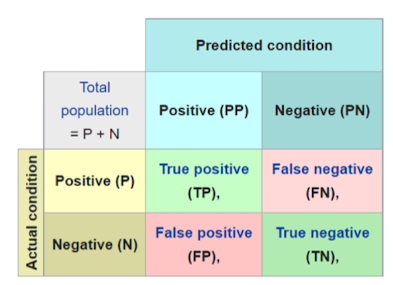
\includegraphics[width=\linewidth]{confusionmatrix}  
\end{minipage}

\subsection{Receiver Operating Characteristics (ROC)}
\begin{minipage}{0,7\linewidth}
	A ROC space is defined by FPR and TPR as x and y axes, respectively, which depicts relative trade-offs between true positives (benefits) and false positives (costs).
	
	Area under the curve is the area under the ROC.  The greater the area under the curve, shows the higher quality of the model.  The greater the area under the curve, the higher the ratio of true positives to false positives.
\end{minipage}
\begin{minipage}{0,3\linewidth}
	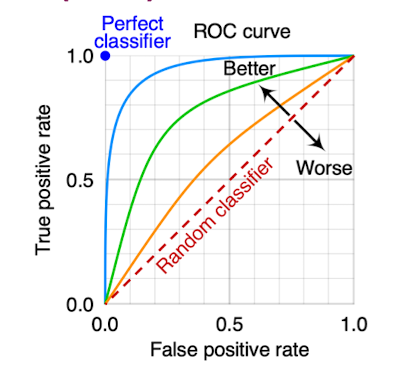
\includegraphics[width=\linewidth]{ROC}  
\end{minipage}


\section{KNN Classification (Unsupervised Learning)}
\subsection{Linear Separability, Decision Boundary}
Two subsets are said to be linearly separable if there exists a hyperplane that separates the elements of each set in a way that all elements of one set resides on the opposite side of the hyperplane from the other set. In 2D plotting, we can depict this through a separation line, and in 3D plotting through a hyperplane. If we have additional information about the structure of the data, we can apply a non-linear transformation.

\subsection{Logistic Regression}
\begin{itemize}[topsep=0pt]
	\itemsep -0.5em
	\item Parametric model (W) $\rightarrow$ Needs training to find optimum W
	\item Computes the probabilities (p), not the class
	\item A suitable threshold needs to be determined (ROC/AUC, FPR vs TPR) to decide the class
	\item Multiple classes can be supported recursively (slow and can result in ambiguity)
	\item Linear decision boundaries between classes
\end{itemize}

\subsection{k-Nearest Neighbors}
A datapoint is known by the company it keeps. It has two Hyperparameters: k value, distance function. \textbf{Advantages:} Easy and simple machine learning model,  Few  hyper parameters to tune. \textbf{Disadvantages:} k should be wisely selected,  Large computation cost during runtime if sample size is large, Not efficient for high dimensional datasets.

\subsubsection{Distance Metric}
There are three different metrics which can be used in the KNN algorithm. We have the distannce $x_{1}=(x_{1,1},x_{1,2},x_{1,n})$ and $x_{2}=(x_{2,1},x_{2,2},x_{2,n})$

\begin{minipage}{0,3\linewidth}
	\textbf{Cosine: (Skalar)}
\[ \frac{x_{1}*x_{2}}{||x_{1}||*||x_{2}||} \] 	 
\end{minipage}
\begin{minipage}{0,3\linewidth}
	\textbf{Manhattan: (Quadrat)}
	\[ \sum_{i=1}^{n} |x_{1,n} - x_{2,n}|\]  
\end{minipage}
\begin{minipage}{0,5\linewidth}
	\textbf{Euclidian: (Kreis)}
 \[ \sqrt{\sum_{i=1}^n (x_{i} - x_{i})^2} \]
\end{minipage}



 
 
 
 
 
 
